\chapter{Real-time implementation}
\label{chp:realtime_implementation}
% Explain:
% - Why a real time system is needed
% - The architecture of the chip
% - How we achieve real time performance by using different specialized tools from the chip

In this chapter, the functionality of the chip is explored, an the general program flow is discussed.

\section{Overview}
% This part will be written last
A big part of the innovation of this thesis is implementing all of the calculations on the chip itself. The chip comes equipped with a radio front-end, two processors and other hardware which must all work in unison to do all of the calculations in time. Before the coding can start, the programmer needs to have a good knowledge of how all of the elements in the chip need to work together.

\section{How it works}
% Why is a real time system needed
In a clinical environment, real-time devices have become indispensable. To give a patient the best care possible, vital signs need to be monitored. These vital signs need to be available right away, because if the patients condition is deteriorating, immediate action is from the utmost importance. There are several examples of real-time clinical measurements. Monitoring of the heart with an ECG, heart rate and oxygen levels in the blood using a pulse-oxygen sensor. But also blood pressure, body temperature and respiration rate can be measured in real-time.

Because this real-time aspect is so important, it also is a big design goal for this project. As can be read in Section~\ref{sec:related_work}, there are some implementations which can measure the vital signs of multiple people using only one radar, but all of those methods are using a post-processing technique. This means that the data is first gathered using the radar and captured with a capture card. At a later stage, all of this data is analyzed and the vital signs are extracted. So there are vital signs measured, but they are available far too late from a clinical point of view. The implementation from this project is focusing on the immediate availability of the vital signs which are being recorded at that moment using the radar. In this chapter the designs, elements and techniques are highlighted to process these relatively large amounts of data using a low power chip.

\section{Building blocks}
\label{sec:building_blocks}
The IWR6843 chip consists of two processors. One is a more generic ARM Cortex R4F processor with a clock speed of 200 MHz. The other one is a Digital Signal Processor (DSP) specific C674x processor, made by TI. These two processors are separated into two sub-systems: the main sub-system and the DSP sub-system. See also Figure~\ref{fig:iwr6843_inner_block_diagram}.

\begin{figure}[t]
\centering
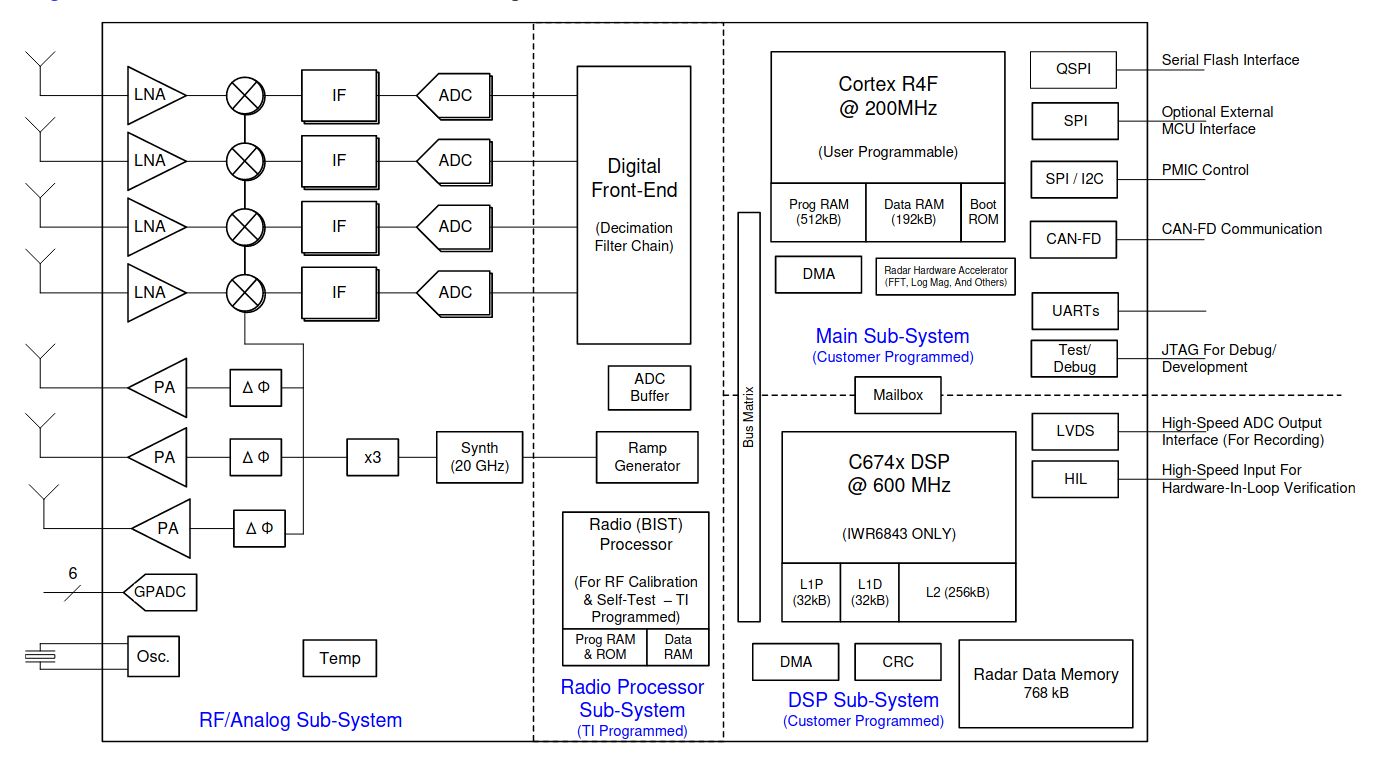
\includegraphics[width=.95\textwidth]{figures/realtime_implementation/iwr6843_inner.png}
\caption{Block diagram of the inner components from the IWR6843.}
\label{fig:iwr6843_inner_block_diagram}
\end{figure}

\subsection{Main sub-system}
The Cortex R4F processor is the more generic all purpose processor in the system. This processor has a managing role in the system. The R4F is connected to all of the communication interfaces, like SPI, I2C, UART and CAN. It is also connected to the radio front-end of the chip. Via a special mailbox system it is also connected to the DSP. 

The main sub-system (MSS) is responsible for all non digital signal processing tasks. It catches the chirp- and frame-interrupts from the radio front-end, and communicates them to the DSP. It also takes care of communicating with external devices. In the case of this project, UART is extensively used to communicate the measurement details with a computer. Another use case for the R4F are more general calculations on the radar data. The DSP takes all of the raw radar data in and processes it to a radar cube. In this radar cube are points in 3 dimensional space, which are detected by the radar. The R4F has also access to this data, and could perform additional algorithms on this data, like object detection, point grouping or even AI techniques.

\subsection{DSP sub-system}
The DSP sub-system (DSS) is responsible for the transformation between the raw ADC radar data and usable data for further processing, for example in a radar cube format. The DSS has also a hardware accelerator build-in, to be able to do specific radar signal processing steps as fast as possible. The Radar Hardware Accelerator (HWA) enables off-loading the burden of certain frequently
used computations in FMCW radar signal processing from the main processor. FMCW radar signal processing involves the use of FFT and log magnitude computations to obtain a radar image across the angle, velocity, and range dimensions. This gives the flexibility of doing common calculations using the HWA, but still design your own algorithms.

The DSP has L1 and L2 caches to store and load calculations quickly. The L3 cache is shared with the MSS, and contains all of the radar data. 

\subsection{Inter-processor communication}
Because the MSS and the DSS are separate processes but must be working in unison, there is a communication technique present in the chip called the \emph{mailbox}. Using this mailbox, messages can be send from one processor to the other, and vice versa. When a message arrives at a processor, an interrupt is triggered and the message can be processed. Another way to use this method is to use it for processor synchronization. Quite often, the two processors need to be in the same state to proceed to the next part of a calculation. When the two processors are synchronized using the mailbox, they both are at a known state in the program flow and can continue with the task at hand. See as an example Figure~\ref{fig:mailbox_principle}. The processors are starting separately, and are doing each their own initialization routine. After that routine is finished, they are waiting on each other (synchronized). Then they can start the program execution at exactly the same time. An example of sending a message from one processor to another is also given in Figure~\ref{fig:mailbox_principle}.

\begin{figure}[t]
\centering
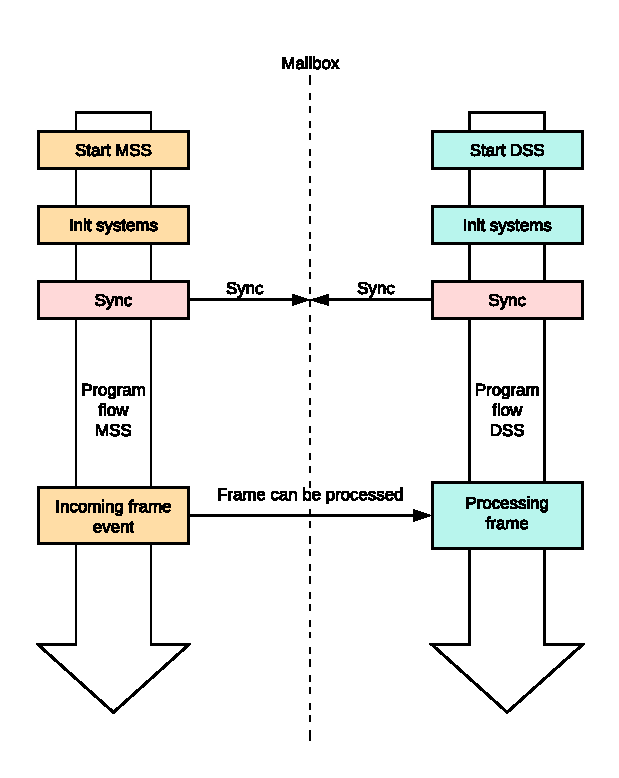
\includegraphics[width=.6\textwidth]{figures/realtime_implementation/Mailbox working principle.pdf}
\caption{Example of the mailbox principle. After startup and initialization, the two processors are synchronized such that they start at the same time. When a frame event ends up at the MSS, it can send a message using the mailbox to the DSS.}
\label{fig:mailbox_principle}
\end{figure}

\section{Implementation}
This section goes into the program flows which make it possible to have real-time vital signs monitoring for multiple persons which are sitting in front of the sensor. A high-level overview can also be found in Figure~\ref{fig:program_flow}.

Like mentioned in Section~\ref{sec:building_blocks}, the IWR6843 contains two processors, one generic ARM processor and one TI DSP. These processors are programmed separately, but the program flow is intertwined, both processors depend on each other to send and receive information. 

\subsection{MSS program flow}
The program starts with an initialization phase, in this phase the processor gets setup to send and receive information from the right locations. The next step is to wait for the CLI input. The IWR6843 receives commands from the connected computer to provide the right parameters for the inner workings of the chip, see also Section~\ref{sec:radar_parameters}. These parameters are processed, checked for errors and are getting send to the right locations. Some parameters are meant for the DSP, some are to program the radio front-end and some are for the MSS itself. After that step, the biggest task from this processor is done. There are two tasks that remain. The interrupts from the radio front-end which signal that a frame has been completed are getting send to the MSS. These messages are getting communicated along to the DSP, where the actual processing can start. All of the radar signal processing and the additional algorithm execution is done on the DSP. This program flow could be optimized a bit to divide the work between the two processors, but for this proof-of-concept design it was easier to do all of the calculations on one processor. When all of the data has been processed by the DSP, the heatmap and all of the vital signs information gets send back to the MSS. The MSS packages this information in a format which can be send over UART and sends this information to the connected computer, where it can be visualized using the GUI.

\subsection{DSS program flow}
The DSP also starts with an initialization phase, just like the MSS. But after that, it is very much a reactionary system. It gets impulses from external sources and reacts accordingly. Once the MSS sends the CLI parameters, it saves them into memory. This action can happen at any time during the runtime of the chip. The real important routine gets called when a signal is received from the MSS that the radar frame has been completed. This means that all of the information is present in memory to start another calculation round. First, the heatmap is generated using the HWA and the raw radar data. When this step is done, the people detection algorithm finds the persons in the room once every 64 frames. This happens only each 64 frames, to stabilize the person detection, persons in the room are in a static position anyway. Now that the positions of the persons in the radar view are known, the DSP proceeds to do a vital signs estimation on each of the persons in view of the sensor. After this has been done, the DSP sends this information back to the MSS.

\subsection{Timing}
For this project, timing is important. For the vital signs estimation to work properly, the system must process radar data at 10 frames per second. This means that each 0.1 second a new radar frame arrives and must be processed before the next frame arrives. The DSP is able to handle this load and always finishes with all the calculations before the next frame is ready. What could have posed a problem, is sending the data back to the computer using UART. The heatmap is 48 azimuth bins wide, 64 range bins long and each bin is 2 bytes. This means $48 \times 64 \times 2 = 6144$ bytes of data which need to be send each 0.1 seconds. The vital signs data is an additional 80 bytes of data, including the packaging of the data 6400 bytes of data need to be send. The UART port being used is running at 921600 baud, which means that 115200 bytes of data can be send each second. Doing the calculations, $6400 / 115200 = 0.056$ seconds. With means that 56\% of the time would be lost just sending the data. The solution to this problem is to use the MSS processor to send the data. This is possible because of the shared address space of the DSP and the MSS. So while the DSP starts doing the calculations for the next frame, the MSS is sending the data from the previous frame back to the computer. See also Figure~\ref{fig:uart_timing}.

\begin{figure}[t]
\centering
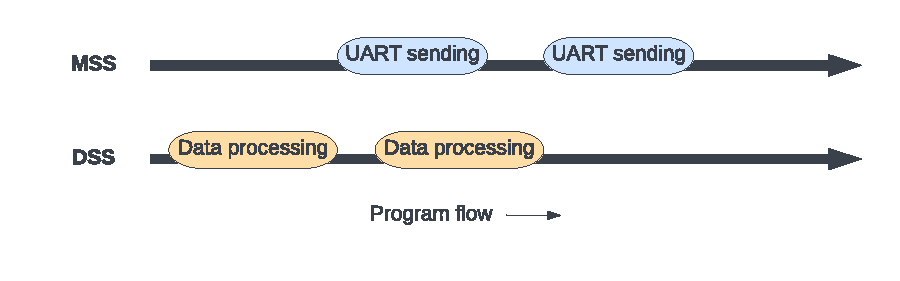
\includegraphics[width=.95\textwidth]{figures/realtime_implementation/timing_diagram.pdf}
\caption{Visual representation of how the two processors are working together to be as efficient as possible.}
\label{fig:uart_timing}
\end{figure}

\begin{figure}[t]
\centering
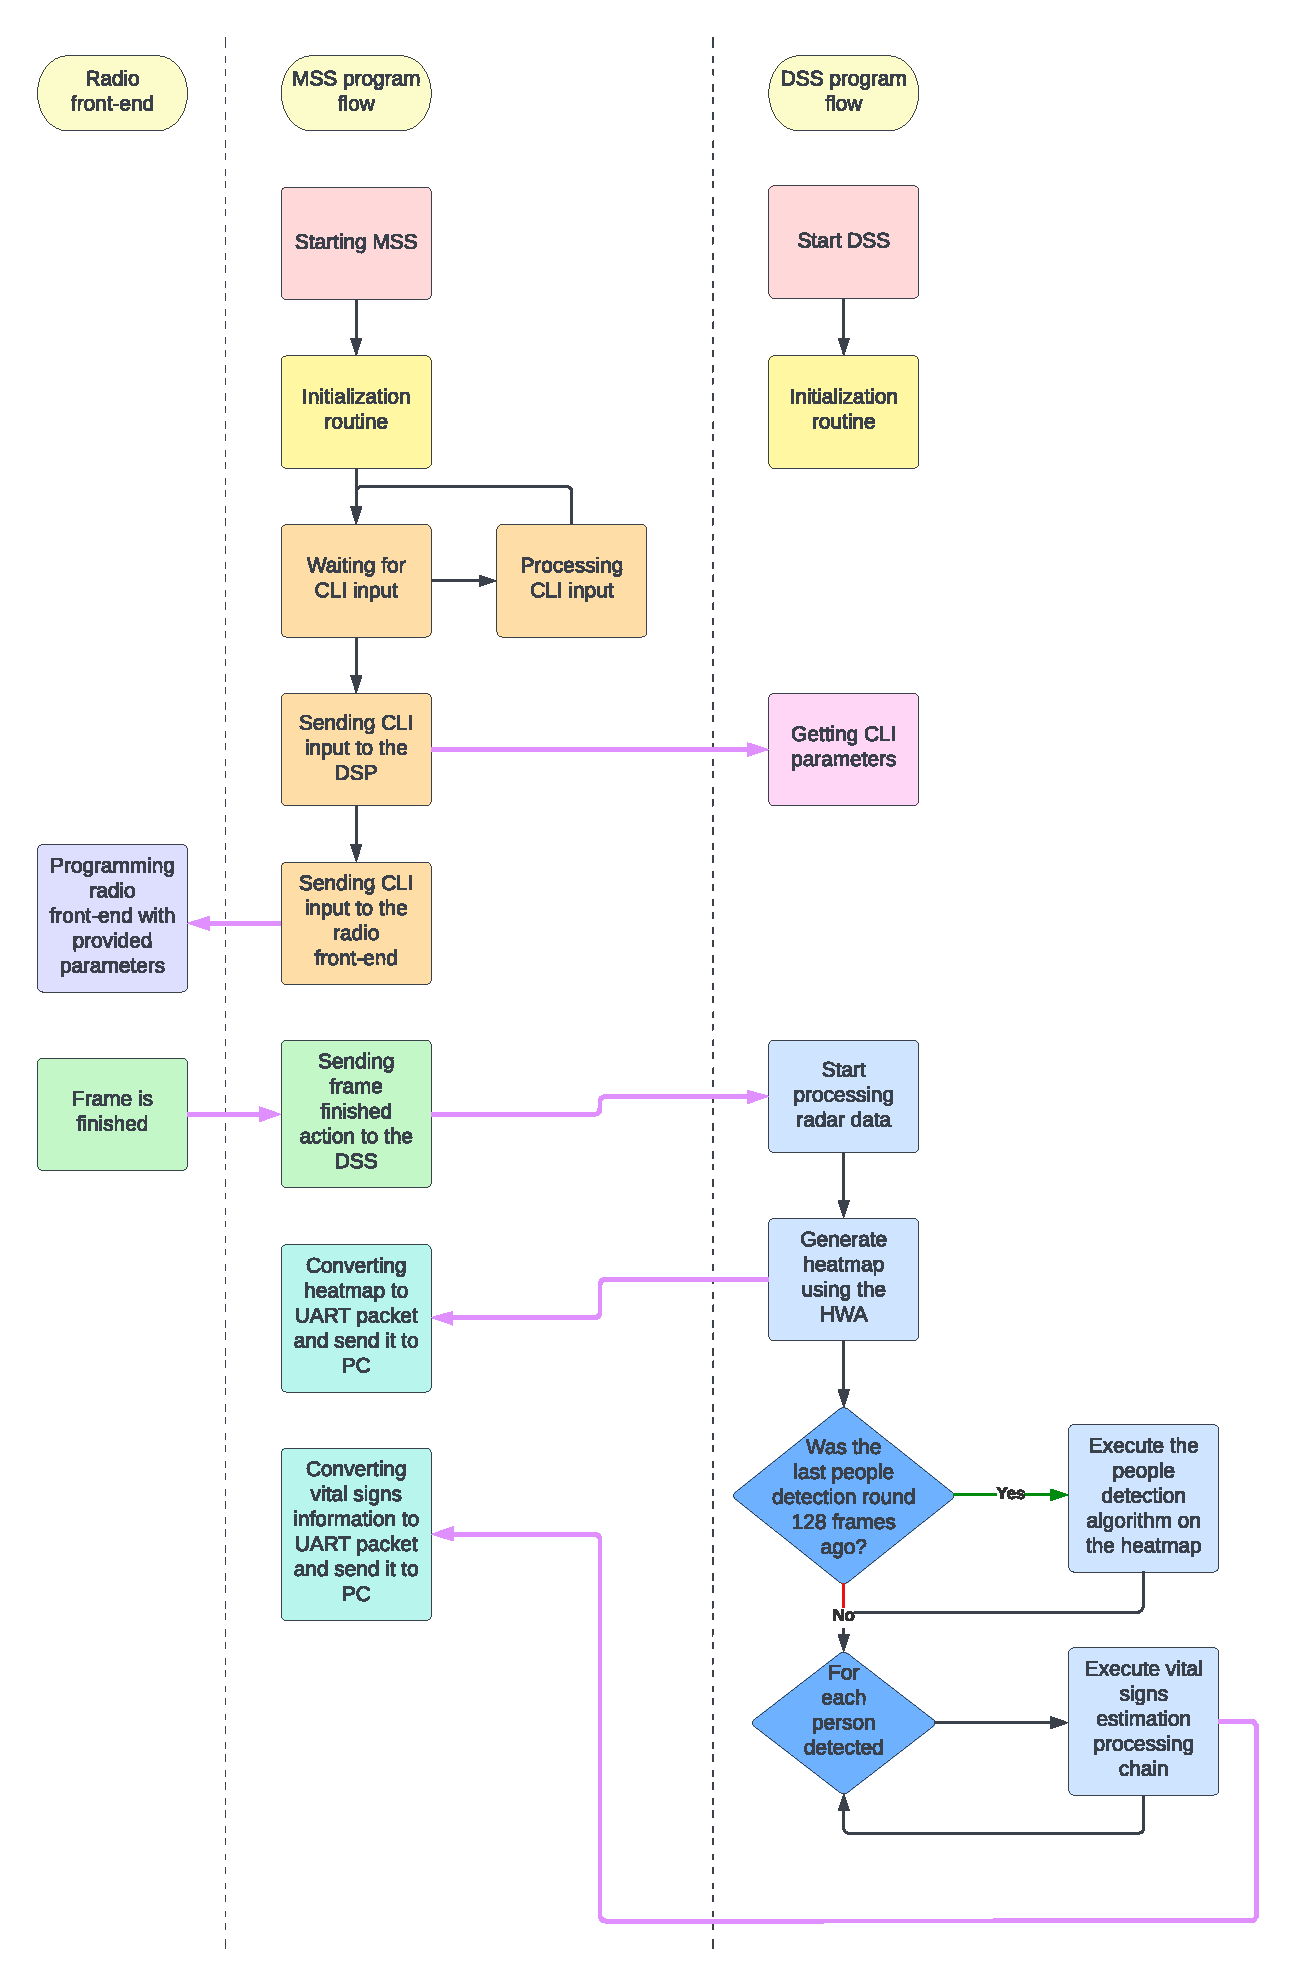
\includegraphics[width=.95\textwidth]{figures/realtime_implementation/Program flow.pdf}
\caption{The program flow from the project in high-level overview. Steps with the same color belong to each other.}
\label{fig:program_flow}
\end{figure}
% Explain:
% - The generic processor
% - The DSP
% - The two processors working together
% - The several hardware accelerators
% - The high-level program flow inside the chip